\chapter{ابزارهای لازم}
	برای تولید یک خروجی مناسب، نیاز به نصب و استفاده از ابزارهای زیر دارید:
	\begin{itemize}
		\item یک توزیع \lr{\LaTeX} مانند \lr{TeXLive}، \lr{MiKTeX} یا \lr{MaxTeX}. لازم به ذکر است که این قالب با استفاده از توزیع \lr{TeXLive 2017} تولید شده‌است.
		\item یک ویرایشگر متن مانند \lr{bidiTeXMaker}، \lr{TeXStudio}، \lr{TeXWorks}، \lr{Notepad++} و مانند آن‌ها. در این مورد، پیشنهاد می‌شود تا از \lr{bidiTeXMaker} یا \lr{TeXWorks} استفاده کنید.
	\end{itemize}

برای \gls{download} \gls{file} \lr{TeXLive 2017}، می‌توانید از آدرس \url{https://www.tug.org/texlive/acquire-iso.html} استفاده نمایید. در صورتی که در شبکه‌ی داخلی دانشگاه حضور دارید؛ توصیه می‌شود تا از آدرس \url{ftp://ftp.vru.ac.ir/Professor/Technical/A.shakiba/} استفاده کنید. لازم به ذکر است که \gls{file} حجیم و در حدود $4$ گیگابایت است. این راهنما بر مبنای راهنمای موجود در سایت پارسی‌لاتک\LTRfootnote{\url{http://www.parsilatex.com/wiki/\rl{راهنمای_نصب_تک‌لایو}}} نوشته شده‌ است.

به منظور یادگیری \gls{typeset} با \lr{\LaTeX} توصیه می‌شود تا از کتاب «مقدمه‌ای نه چندان کوتاه بر \lr{\LaTeX}»، ترجمه‌ی آقای مهدی امیدعلی\LTRfootnote{\url{https://www.ctan.org/tex-archive/info/lshort/persian}} استفاده نمایید. همچنین، می‌توانید در کارگاه‌های آموزشی دانشکده‌ی علوم ریاضی در ابتدای هر ترم، شرکت کنید.

\begin{figure}
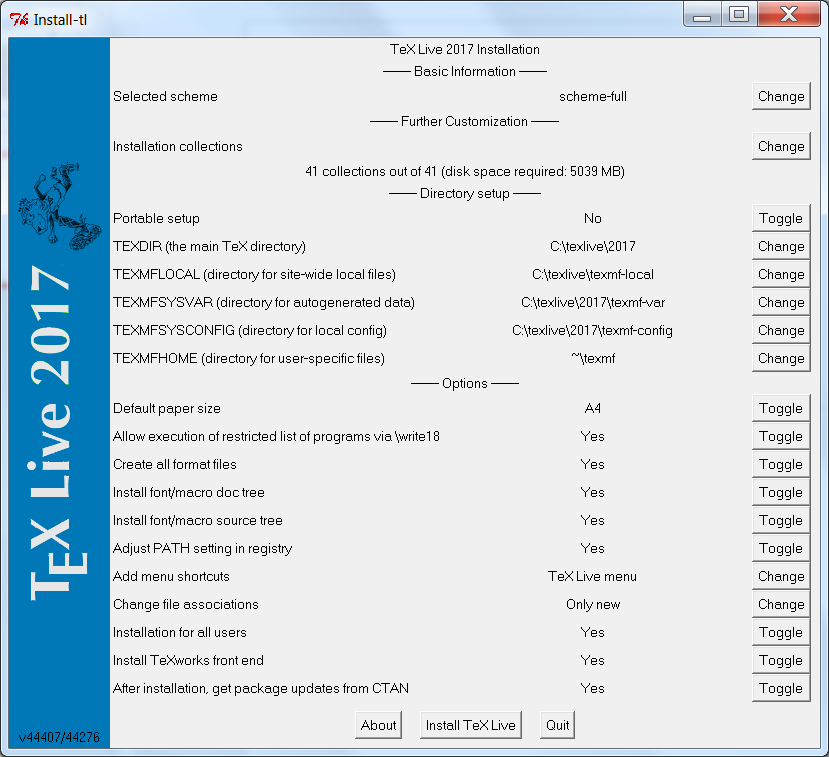
\includegraphics[width=.7\textwidth]{figs/texlive2017.png} 
\caption{پنجره‌ی نصب \lr{TeXLive 2017}.}
\end{figure}